\documentclass[a4paper, twoside]{article}

%%%%%%% multilingual
\usepackage[english]{babel}
\usepackage[applemac]{inputenc}
\usepackage[cyr]{aeguill}
\usepackage{xspace}
% ----- end of multilingual

\usepackage[backref,breaklinks]{hyperref} % links, toc
\usepackage{graphics}
\usepackage{fancyhdr} % headers

\usepackage{hyphenat} % c_variables hyphenation

\setlength{\parskip}{1ex}

\begin{document}

%%%%% definitions
\newcommand{\theversion}{$Revision: 1.6 $}

\newcommand{\theday}{9th}
\newcommand{\themonth}{May}
\newcommand{\theyear}{2008}
\newcommand{\thedate}{\theday\ \themonth\ \theyear\ (\theversion)}

\newcommand{\separation}{\vspace{1ex}}

\newcommand{\rta}{\textit{RTA}}
\newcommand{\htk}{\textit{HTK}}
\newcommand{\atb}{\textit{Auditory Toolbox}}
\newcommand{\lpc}{\textit{LPC}}
\newcommand{\mfcc}{\textit{MFCC}}
\newcommand{\yin}{\textit{yin}}
\newcommand{\Yin}{\textit{Yin}}
\newcommand{\del}{\textit{delta}}
\newcommand{\Del}{\textit{Delta}}
\newcommand{\ddel}{\textit{delta-delta}}

\newcommand{\thebigtitle}{\rta\ Documentation\\
  Using the \rta\ library to compute on-line sound descriptors}

\newcommand{\thetitle}{\rta\ documentation for sound descriptors}

% \renewcommand{\contentsname}{}



% ---- end of definitions


%%%%%%%%%%% headers and footers %%%%%%%%%%%%%%%

% Headers and footers personalisation using the `fancyhdr' package
\fancyhf{} % Clear all fields

\fancyhead[L]{\thetitle}
\fancyhead[C]{}
\fancyhead[R]{\theversion}

\fancyfoot[C]{\thepage}

\pagestyle{fancy}
%% ------ end of headers and footers

\title{\thebigtitle}

\author{Jean-Philippe Lambert}
\date{\thedate}

\maketitle

{
  % \setcounter{tocdepth}{1}
  \setlength{\parskip}{0ex}
  \tableofcontents
  \listoffigures
  % \setcounter{tocdepth}{3}
  % \vspace{1ex}
}


\section{Doxygen: Code self-contained documentation}
\label{sec:doxygen}

The \rta\ library is documented within the code, using the
\textit{Doxygen} format. This is the reference documentation. To
generate \textit{HTML} and \textit{LaTeX} output, use the command
\texttt{doxygen Doxyfile} within the \texttt{rta} directory.  The
\textit{HTML} documentation will then be accessible from
\texttt{rta/doc/html/index.html}. To compile a \textit{PDF} document,
use the command \texttt{make} within the \texttt{rta/doc/latex}
directory, which is generated by the previous command.

\section{Generalities}
\label{sec:generalities}

The \rta\ library is frame-based, which means that for any vectors of
samples, a set of descriptors can be computed without adding any
delay. A noticeable exception to this is the \del\ (and
\ddel) computation, as it is based on more than on frame.

There are two variants of each function, one being \texttt{\_stride}
post-fixed. It allows to directly access interleaved data without
copying them (like a stereophonic samples vector). However, using a
big \emph{stride} value may lead to a bad usage of the memory cache.

Any index starts at 0.

Some functions require an initialisation before any processing, in
order to pre-calculate what will not depend on the incoming
frame. Every allocation must be done before anything else, outside of
the functions themselves except mentioned otherwise.

Some descriptors can be computed by several functions, and the results
may slightly differ for several reasons: the functions does not rely
on the same algorithms and the signal used for the computation may
differ (due to windowing, filtering, etc.). The auto-correlation from
\yin\ and from the \lpc\ are not the same and there is a
lot of ways to get the energy: from \yin, as the sum of the
squares of the samples, from \lpc, or as the first
\mfcc coefficient.

\section{Library configuration}
\label{sec:configuration}

A file named \texttt{rta\_configuration.h} must be present within your
sources in order to use the \rta\ library. An empty file means that
the defaults settings are used for the compilation. 

Instead of using the \texttt{malloc}, \texttt{realloc} and
\texttt{free} functions from the \texttt{stdlib.h}, one can
respectively define \texttt{rta\_malloc}, \texttt{rta\_realloc}
and \texttt{rta\_free}.

The floating-point precision can be simple, double or long
double, according to the definition of \texttt{RTA\_REAL\_TYPE} to
respectively \texttt{RTA\_FLOAT\_TYPE}, \texttt{RTA\_DOUBLE\_TYPE} or
\texttt{RTA\_LONG\_DOUBLE\_TYPE}. The constants in
\texttt{rta\_float.h} are then redefined according to the proper type
from \texttt{float.h}. The same applies to the functions in
\texttt{rta\_math.h} from \texttt{math.h}.

Note that the long double precision is not supported when using the
Apple's VecLib by setting \texttt{RTA\_USE\_VECLIB} to 1.

% \section{Dataflow}
% \label{sec:dataflow}

\begin{figure}[!hbt]
  \centering
  \resizebox{12cm}{!}{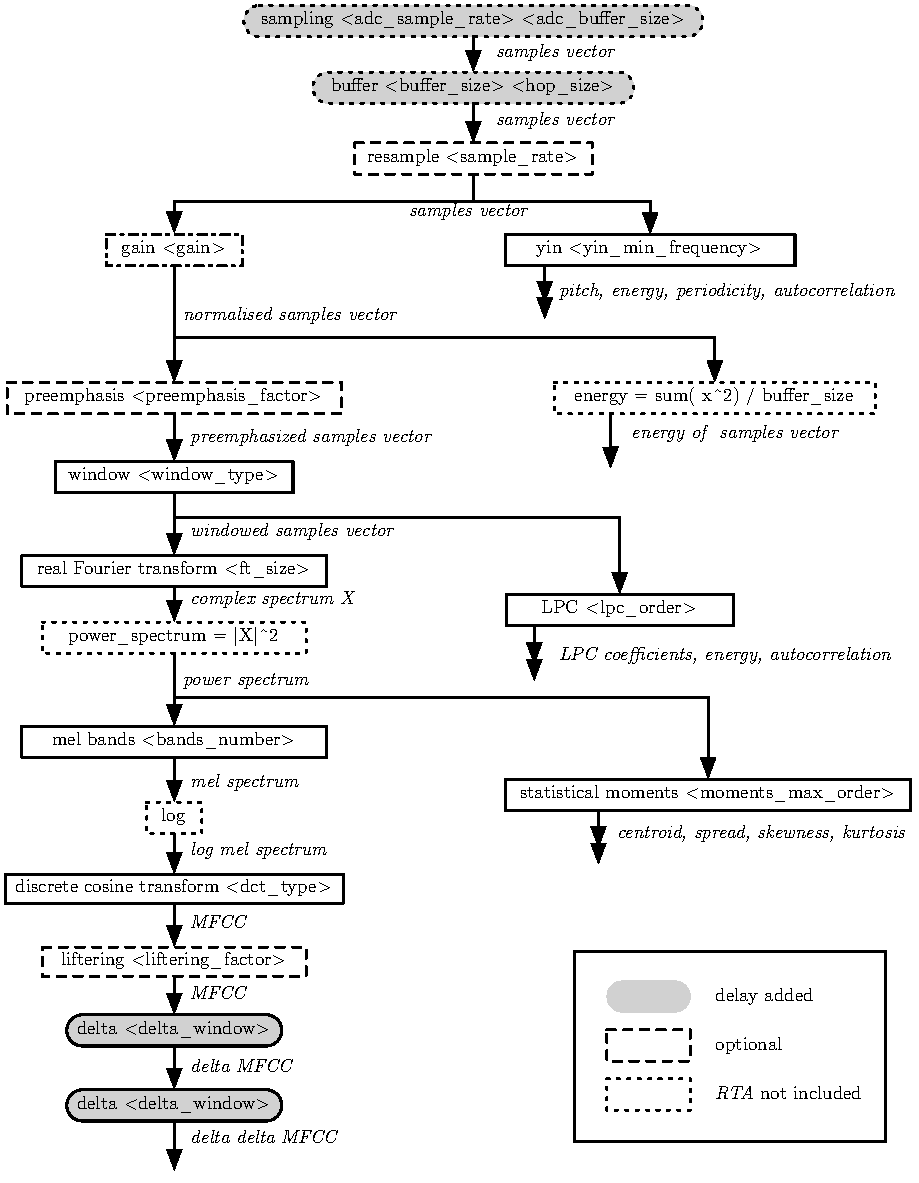
\includegraphics{rta_dataflow}}
  \caption[Sound descriptors data-flow]{Sound descriptors data-flow}
  \label{fig:dataflow}
\end{figure}

\section{Descriptors based on a vector of samples}
\label{sec:samples_vector_descriptors}

The vector of samples is characterised by its sample-rate and its
size. Moreover, to use sizes larger than those provided by the
sound card (e.g. for Fourier transforms), the hop-size gives the number
of samples between two consecutive vectors that overlap if the hop-size
is smaller than the vector-size.

\subsection{Re-sampling}
\label{sec:resampling}

Down-sampling a signal is interesting to lower the further
computations, especially for the computational-intensive algorithms,
like \yin. It can helps to concentrate on a range of the
spectrum where the information is pertinent for the analysis: the
\lpc\ (which is linear, as its name suggests it) finds poles
and zeros to fit the whole spectrum; to keep the results under 5 kHz,
we simply use a sample-rate of 11 kHz. If the original signal
sample-rate is 44 kHz, we can use the function
\texttt{rta\_downsample\_int\_mean} with a factor of 4. This function
implies a low-pass filtering. The function
\texttt{rta\_downsample\_int\_remove} can produce aliasing if the
original signal contains information above the resulting
sample-rate. Note that the resulting samples vector-size is smaller,
according to the given factor.

\subsection{\Yin}
\label{sec:yin}

The \yin\ algorithm computes the periodicity of a samples
vector, finding its most probable \emph{lag}. To get the period in Hz,
on simply multiply this lag by the input vector sample-rate.

Note that the \yin\ algorithm operates on a non-windowed
samples vector. As it can be computational-intensive, a down-sampling
of the incoming vector is often performed: to track a pitch below 1
kHz, one can use a sampling-rate of 11 kHz, or even 5.5 kHz, depending
on the results quality request. One can then check the \emph{absolute
  minimum} found, which gives the \emph{periodicity} as long as the
absolute minimum is positive:
$$periodicity = 1 - \sqrt{absolute\_minimum}$$

Before computing anything, a new \yin\ structure must be
allocated and filled with the \texttt{rta\_yin\_setup\_new}
function. It will be released by the function
\texttt{rta\_yin\_setup\_delete}. (The auto-correlation result vector
must also be allocated beforehand, like any results vector.)

\subsection{Gain and integer--float conversion}
\label{sec:gain}

The samples are generally coded by floating-points number over 32
bits, within the range $[-1.0, 1.0]$. To convert them into 16 bits
signed integers (which is the format used by some systems, like
\htk), one can apply a simple gain of $2^{15}$ by multiplying
every sample.

\subsection{Pre-emphasis}
\label{sec:preemphasis}

The pre-emphasis is a simple first-order difference between a current
sample and the previous one (weighted by a factor):
$$s(n) = s(n) - f \times s(n-1)$$

It is often used for voice analysis with a factor of 0.97 as it
reduces the low frequencies while raising the high frequencies, thus
amplifying the contrast.

\subsection{Windowing}
\label{sec:windowing}

If the samples vector-size is known, it is possible to pre-calculate
the weights that will be used to apply a given function. The function
\texttt{rta\_window\_hamming\_weights} computes a \textit{Hamming}
window while the function \texttt{rta\_window\_hann\_weights} computes
a \textit{von Hann} window. These (or any weights vector) can be
applied with the \texttt{rta\_window\_apply} function. The
\texttt{\_in\_place} post-fixed functions change the input samples
vector values directly.

If the samples vector-size is not known in advance, one can still
apply the window using the \texttt{rta\_window\_rounded\_apply}
function. There is no interpolation, then. The weights vector indexes
are simply scaled and rounded: this is efficient but the rounding
error may be unacceptable if the size of the weights vector is too
small comparing with the samples vector size. It is also possible to
compute and apply a window on the fly, with the functions
\texttt{rta\_window\_hann\_apply} and
\texttt{rta\_window\_hamming\_apply}.


\subsection{Linear predictive coefficients (\lpc)}
\label{sec:lpc}

The \texttt{rta\_lpc} function calculates the linear predictive
coefficients (\lpc) for a samples vector, using an auto-correlation
and a \textit{Levinson-Durbin} decomposition. Note that the \lpc\
order is one value less than the \lpc\ size.

The first \lpc\ coefficient is always 1 and is often replaced (e.g. in
\htk) by the prediction error, which gives the energy of the samples
vector. If the \lpc\ is computed on overlapping samples vectors, they
are often windowed in order for the coefficients to evolve smoothly
from frame to frame, and the energy is then reduced (by a constant
factor depending on the window).

\section{Descriptors based on the power spectrum}
\label{sec:power_spectrum_descriptors}

Some descriptors are based on the power spectrum of a samples
vector. The samples vector is first windowed. Then a real
\textit{Fourier} transform is applied, giving a complex spectrum. The
power spectrum is the square of the magnitude of the complex spectrum.

\subsection{Real Fourier transform}
\label{sec:fft}

Before computing a real \textit{Fourier} transform, a new real
\textit{Fourier} transform setup must be allocated and filled with the
\texttt{rta\_fft\_real\_setup\_new} function, with the type
\texttt{real\_to\_complex\_1d}. It will be released by the
function \texttt{rta\_fft\_setup\_delete}. The function
\texttt{rta\_fft\_execute} applies the \textit{Fourier} transform
to a samples vector.

The transform size must be a power of 2. If the transform size is
bigger than the actual samples vector, it is then padded with zeros.

By convention (e.g. \htk), no scale is applied to this direct
transform. The inverse of the transform size can later be applied to
the inverse transform in order to obtain the identity transform.

\subsection{Complex spectrum to power spectrum }
\label{sec:power_spectrum}

The power spectrum is the square of the magnitude the complex
spectrum.
% $$ power\_spectrum = |X|^2$$
Its size is half the size of the \textit{Fourier} transform plus one
(the last element corresponds to the \textit{Nyquist} frequency). To
get a correspondence between the power spectrum index and the
corresponding frequency, one can apply a simple ratio between the
maximum frequency (which is half of the sample-rate) and the maximum
index (which is half of the \textit{Fourier} transform size, as all
the indexes start at 0):
$$ frequency = index \frac{sample\_rate}{transform\_size}$$

\subsection{Statistical moments}
\label{sec:moments}

The statistical moments can be computed from any samples vector, as
long as the weights are positive, as they represent the probability of
the random variables to appear. The power spectrum conforms to this, as
any value is positive, but not the amplitude spectrum (if not
translated above 0). The same applies for the moments of the mel
bands.

The moments are calculated over the indexes and weighted by the input
values. They will be normalised by the sum of the input values in order
to get the indexes probability. Note that all moments (but the first)
are centred. Any moment above the second can be standardised. 

The moments described hereafter describe the power spectrum moments.

\subsubsection{Centroid}
\label{sec:centroid}

The spectral centroid is the first moment over the indexes weighted by
the vector of power spectrum values. It is computed by
\texttt{rta\_weighted\_moment\_1\_indexes}. The result unit is
$index$ (of the power spectrum, starting at 0). This function
returns also the input sum as it can be used in further calculations.
$$ m_1 = centroid = \frac {\sum_i i \times input(i)}
{\sum_i input(i)} $$


\subsubsection{Spread and deviation}
\label{sec:spread}

The spectral spread is the second central moment over the indexes
weighted by the vector of power spectrum values. It is computed by
\texttt{rta\_weighted\_moment\_2\_indexes}. The result unit is
$index^2$ (of the power spectrum, starting at 0).
$$ m_2 = spread = \frac {\sum_i (i - centroid )^2 \times input(i)}
{\sum_i input(i)} $$

The standard deviation is $std = \sqrt{spread}$.

\subsubsection{Skewness}
\label{sec:skewness}

The spectral skewness is the third standard central moment over the
indexes weighted by the vector of power spectrum values. It is
computed by \texttt{rta\_std\_weighted\_moment\_3\_indexes}. The
result is without unit.
$$ m_{3std} = skewness = \frac {\sum_i (i - centroid )^3 \times input(i)}
{std^3 \sum_i input(i)} $$

\subsubsection{Kurtosis}
\label{sec:kurtosis}

The spectral kurtosis is the fourth standard central moment over the
indexes weighted by the vector of power spectrum values. It is
computed by \texttt{rta\_std\_weighted\_moment\_4\_indexes}. The
result is without unit.
$$ m_{4std} = kurtosis = \frac {\sum_i (i - centroid )^4 \times input(i)}
{std^4 \sum_i input(i)} $$

Note that the kurtosis is often defined as the fourth cumulant divided
by the square root of the variance, which gives $kurtosis =
\frac{m_4}{std^4} - 3$.  This function does not include the ``$- 3$''
term.

\section{Descriptors based on the mel bands}
\label{sec:mel_descriptors}

The mel scale can be derived from the frequencies in hertz. The
conversion functions are in \texttt{rta\_mel.h}. They are based on two
slightly different formulas, according to \htk\ or the \atb\ with the
respective suffix \texttt{\_htk} or \texttt{\_slaney}.

The power spectrum is integrated into several bands, according again
to \htk\ or the \atb. The integration
window peak is 1 for \htk, while the sum of any channel is 1
for the \atb.

In order to reproduce the results of one of these tools, one must
obviously choose the desired variant among the whole computation
process.

\subsection{Mel bands}
\label{sec:mel}

The mel bands integration is done in the magnitude ($abs$) or the
power ($abs^2$) domain, using respectively the function
\texttt{rta\_spectrum\_to\_bands\_abs} or
\texttt{rta\_spectrum\_to\_bands\_square\_abs}. This respectively
gives
$$ mel\_bands = weights\_matrix \times spectrum $$
or
$$ mel\_bands = (weights\_matrix \times \sqrt{spectrum})^2 $$
The latter is the default (for \htk\ and \atb) but it involves more
computation.

The matrix to multiply the power spectrum vector with, in order to
obtain the mel bands, must be computed beforehand, using the
\texttt{rta\_spectrum\_to\_mel\_bands\_weights} function.


\subsection{Mel-frequency cepstral coefficients (\mfcc)}
\label{sec:mfcc}

First, the logarithm of the mel bands values is taken. In order to
avoid $log(0)$, one can add a very small value to the mel bands
values before taking the log.

Then a cepstrum is computed for the log of the mel spectrum, using a
discrete cosine transform (\textit{DCT}) of type II. \htk\
uses an orthogonal but not unitary transform, while the \atb\ uses an
orthogonal and unitary transform. First, a weights matrix is
constructed with the function \texttt{rta\_dct\_weights} and it is
then applied to the mel bands vector using the function
\texttt{rta\_dct}. The coefficients obtained are the \mfcc.

The \mfcc\, as any \textit{DCT} coefficients, are ordered by the order
of importance to model the spectrum. However, one can need to modify
them (for visualisation or further processing) using the liftering
functions in \texttt{rta\_lifter.h}. These functions are provided for
the \htk\ or \atb\ compatibility.

\subsection{\Del\ and \ddel\  \mfcc}
\label{sec:delta_mfcc}

The function \texttt{rta\_delta} computes a simple linear slope on a
sequence of fixed-rate sampled data (the frames). The \del\ values
correspond to the mid-point frame (which is not used, by the
way). \emph{It means that the \del\ values are not those of the last
  frame}. Considering the filter-size, which is the size of the
sequence taken into account, the delay (in frames) introduced is half
of the filter-size (rounded down as it is always odd).

Note that the \htk\ \texttt{DELTAWINDOW} variable is not the same as
the filter-size (the same applies for the \texttt{ACCWINDOW}
variable):
$$ filter\_size = 1 + 2 \times DELTAWINDOW $$

Beforehand, a matrix of weights to multiply the sequence vector with
is constructed by the function \texttt{rta\_delta\_weights}. A
normalisation factor, computed by the function
\texttt{rta\_delta\_normalization\_factor} gives \del\ values, which
are independent of the filter-size. The normalisation factor can be
applied directly to the weights matrix but the rounding errors may be
unacceptable when using the simple floating-point precision.

Applying the \del\ computation again gives the \ddel\ values,
\emph{adding a new delay of half of the \ddel\ filter-size}.

\end{document}

%%% Local Variables: 
%%% ispell-local-dictionary: "en_GB" 
%%% End:
